\\
\newpage
\section{SENSOR DE VELOCIDAD}
Dispositivo que mide la rapidez con la que un objeto se mueve. Puede basarse en principios ópticos, magnéticos o mecánicos para calcular la velocidad de giro o desplazamiento.
Sensor automotriz de velocidad y transmisión.\autoref{fig:sensor de velocidad}
\begin{figure}[h]
	\centering
	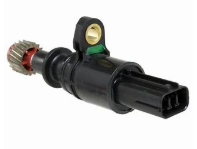
\includegraphics[width=0.3\linewidth]{img/sensor de velocidad}
	\caption{Sensor de velocidad}
	\label{fig:sensor de velocidad}
\end{figure}

\section*{TACOMETRO}
Sensor que mide la velocidad de rotación de un eje o motor, generalmente en revoluciones por minuto (RPM). Puede ser mecánico, óptico o basado en efecto Hall.

\section*{SENSOR DE EFECTO HALL}
Estos sensores detectan la velocidad midiendo cambios en el campo magnético generado por un imán o un objeto ferroso en movimiento. Son ampliamente utilizados en aplicaciones automotrices, como la medición de la velocidad de las ruedas en los sistemas de frenos antibloqueo, y para medir corriente eléctrica.

\begin{figure}[h]
	\centering
	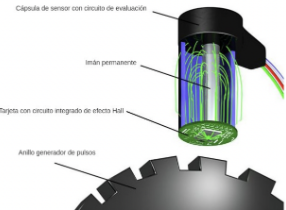
\includegraphics[width=0.3\linewidth]{img/HALL}
	\caption{Sensor de velocidad}
	\label{fig:HALL}
\end{figure}


